\documentclass[aspectratio=169]{beamer}
\usepackage[utf8]{inputenc}
\usepackage[english]{babel}
\usepackage{listings}
\usepackage{xcolor}
\usepackage{tikz}
\usepackage{tcolorbox}
\usetikzlibrary{shapes,arrows,positioning,shadows}

% Definizione simboli alternativi
\newcommand{\faCheck}{$\checkmark$}
\newcommand{\faTimes}{$\times$}
\newcommand{\faInfoCircle}{[i]}
\newcommand{\faExclamationTriangle}{[!]}
\newcommand{\faShieldAlt}{[*]}
\newcommand{\faCheckSquare}{[$\checkmark$]}

% Tema e colori
\usetheme{Madrid}
\usecolortheme{default}
\definecolor{darkblue}{RGB}{0,51,102}
\definecolor{lightblue}{RGB}{51,153,255}
\definecolor{codegreen}{rgb}{0,0.6,0}
\definecolor{codegray}{rgb}{0.5,0.5,0.5}
\definecolor{codepurple}{rgb}{0.58,0,0.82}
\definecolor{backcolour}{rgb}{0.95,0.95,0.92}

\setbeamercolor{structure}{fg=darkblue}
\setbeamercolor{title}{fg=white,bg=darkblue}
\setbeamercolor{frametitle}{fg=white,bg=darkblue}

% Configurazione listing per PHP
\lstdefinestyle{phpstyle}{
	language=PHP,
	backgroundcolor=\color{backcolour},   
	commentstyle=\color{codegreen},
	keywordstyle=\color{blue}\bfseries,
	numberstyle=\tiny\color{codegray},
	stringstyle=\color{codepurple},
	basicstyle=\ttfamily\footnotesize,
	breakatwhitespace=false,         
	breaklines=true,                 
	captionpos=b,                    
	keepspaces=true,                 
	numbers=left,                    
	numbersep=5pt,                  
	showspaces=false,                
	showstringspaces=false,
	showtabs=false,                  
	tabsize=2,
	frame=single,
	rulecolor=\color{black}
}

\lstset{style=phpstyle}

\title{PDO: PHP Data Objects}
\subtitle{Accesso sicuro ai database MySQL}
\author{Prof. Massimo Fedeli}
\institute{IIS Fermi Sacconi Ceci - Ascoli Piceno}
\date{\today}

\begin{document}
	
	% Slide 1 - Titolo
	\begin{frame}
		\titlepage
	\end{frame}

	
	% SEZIONE 1: Introduzione
	\section{Introduzione a PDO}
	
	% Slide 3
	\begin{frame}{Cos'è PDO?}
		\begin{columns}
			\column{0.6\textwidth}
			\textbf{PHP Data Objects (PDO)} è un'estensione che fornisce:
			\begin{itemize}
				\item Interfaccia \textbf{unificata} per l'accesso ai database
				\item Supporto per \textbf{12+ database} diversi (MySQL, PostgreSQL, SQLite, Oracle, etc.)
				\item Meccanismi di \textbf{sicurezza} integrati
				\item \textbf{Prepared statements} nativi
				\item Gestione avanzata degli \textbf{errori}
			\end{itemize}
			
			\column{0.35\textwidth}
			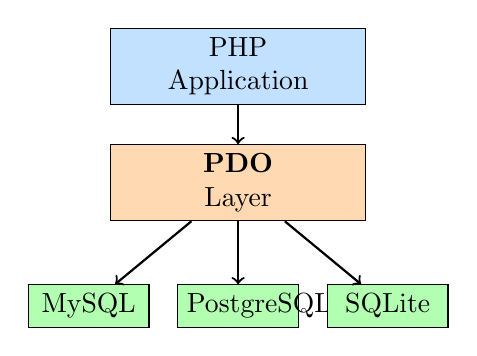
\begin{tikzpicture}[scale=0.8]
				\node[rectangle, draw, fill=lightblue!30, text width=3cm, align=center] (php) {PHP\\Application};
				\node[rectangle, draw, fill=orange!30, text width=3cm, align=center, below=0.5cm of php] (pdo) {\textbf{PDO}\\Layer};
				\node[rectangle, draw, fill=green!30, text width=1.3cm, align=center, below left=0.8cm and -0.5cm of pdo] (mysql) {MySQL};
				\node[rectangle, draw, fill=green!30, text width=1.3cm, align=center, below=0.8cm of pdo] (pgsql) {PostgreSQL};
				\node[rectangle, draw, fill=green!30, text width=1.3cm, align=center, below right=0.8cm and -0.5cm of pdo] (sqlite) {SQLite};
				\draw[->, thick] (php) -- (pdo);
				\draw[->, thick] (pdo) -- (mysql);
				\draw[->, thick] (pdo) -- (pgsql);
				\draw[->, thick] (pdo) -- (sqlite);
			\end{tikzpicture}
		\end{columns}
	\end{frame}
	
	% Slide 4
	\begin{frame}{Perché usare PDO?}
		\begin{tcolorbox}[colback=green!5,colframe=green!40!black,title=\faCheck~Vantaggi di PDO]
			\begin{enumerate}
				\item \textbf{Sicurezza}: protezione nativa contro SQL Injection
				\item \textbf{Portabilità}: codice riutilizzabile su diversi DBMS
				\item \textbf{Prestazioni}: prepared statements più veloci per query ripetute
				\item \textbf{Flessibilità}: modalità di fetch personalizzabili
				\item \textbf{Transazioni}: supporto completo per BEGIN, COMMIT, ROLLBACK
				\item \textbf{OOP}: approccio orientato agli oggetti
			\end{enumerate}
		\end{tcolorbox}
	\end{frame}
	
	% Slide 5
	\begin{frame}{PDO vs mysqli}
		\begin{table}
			\small
			\begin{tabular}{|l|c|c|}
				\hline
				\textbf{Caratteristica} & \textbf{PDO} & \textbf{mysqli} \\
				\hline
				Database supportati & 12+ & Solo MySQL \\
				\hline
				API & Solo OOP & OOP + Procedurale \\
				\hline
				Named parameters & \textcolor{green}{\faCheck} & \textcolor{red}{\faTimes} \\
				\hline
				Prepared statements & \textcolor{green}{\faCheck} & \textcolor{green}{\faCheck} \\
				\hline
				Portabilità & Eccellente & Limitata \\
				\hline
				Curva apprendimento & Media & Bassa \\
				\hline
				Performance & Ottima & Ottima \\
				\hline
			\end{tabular}
		\end{table}
		
		\vspace{0.3cm}
		\alert{\textbf{Raccomandazione}}: PDO per nuovi progetti per maggiore flessibilità
	\end{frame}
	
	% SEZIONE 2: Connessione
	\section{Connessione al Database}
	
	% Slide 6
	\begin{frame}[fragile]{Connessione Base}
		\begin{lstlisting}
			<?php
			// Parametri di connessione
			$host = 'localhost';
			$dbname = 'scuola';
			$username = 'root';
			$password = '';
			
			try {
				// Creazione oggetto PDO
				$pdo = new PDO(
				"mysql:host=$host;dbname=$dbname;charset=utf8mb4",
				$username,
				$password
				);
				
				echo "Connessione riuscita!";
				
			} catch (PDOException $e) {
				die("Errore connessione: " . $e->getMessage());
			}
			?>
		\end{lstlisting}
	\end{frame}
	
	% Slide 7
	\begin{frame}{Anatomia del DSN}
		\begin{tcolorbox}[colback=blue!5,colframe=blue!40!black,title=DSN - Data Source Name]
			\texttt{mysql:host=localhost;dbname=scuola;charset=utf8mb4}
		\end{tcolorbox}
		
		\begin{description}
			\item[\texttt{mysql:}] Driver del database (mysql, pgsql, sqlite, etc.)
			\item[\texttt{host=}] Indirizzo del server database
			\item[\texttt{dbname=}] Nome del database
			\item[\texttt{charset=}] Codifica caratteri (sempre utf8mb4 per MySQL)
		\end{description}
		
		\vspace{0.3cm}
		Altri parametri opzionali:
		\begin{itemize}
			\item \texttt{port=3306} - Porta personalizzata
			\item \texttt{unix\_socket=/path/to/socket} - Socket Unix
		\end{itemize}
	\end{frame}
	
	% Slide 8
	\begin{frame}[fragile]{Opzioni di Connessione}
		\begin{lstlisting}
			<?php
			$options = [
			// Modalita' errore: eccezioni
			PDO::ATTR_ERRMODE => PDO::ERRMODE_EXCEPTION,
			
			// Fetch mode predefinito
			PDO::ATTR_DEFAULT_FETCH_MODE => PDO::FETCH_ASSOC,
			
			// Disabilita emulazione prepared statements
			PDO::ATTR_EMULATE_PREPARES => false,
			
			// Connessione persistente (opzionale)
			PDO::ATTR_PERSISTENT => false
			];
			
			$pdo = new PDO($dsn, $username, $password, $options);
			?>
		\end{lstlisting}
		
		\alert{\textbf{Importante}}: Configurare sempre \texttt{ERRMODE\_EXCEPTION}!
	\end{frame}
	
	% Slide 9
	\begin{frame}[fragile]{Gestione Errori: Le Tre Modalità}
		\begin{columns}
			\column{0.5\textwidth}
			\textbf{1. ERRMODE\_SILENT}
			\begin{lstlisting}[basicstyle=\ttfamily\tiny]
				// Nessun errore mostrato
				// Controllo manuale
				if (!$stmt->execute()) {
					print_r($stmt->errorInfo());
				}
			\end{lstlisting}
			
			\textbf{2. ERRMODE\_WARNING}
			\begin{lstlisting}[basicstyle=\ttfamily\tiny]
				// Warning PHP standard
				// Non interrompe esecuzione
			\end{lstlisting}
			
			\column{0.5\textwidth}
			\textbf{3. ERRMODE\_EXCEPTION} \textcolor{green}{\faCheck}
			\begin{lstlisting}[basicstyle=\ttfamily\tiny]
				try {
					$stmt = $pdo->query($sql);
				} catch (PDOException $e) {
					echo "Errore: ";
					echo $e->getMessage();
				}
			\end{lstlisting}
			
			\vspace{0.2cm}
			\alert{\textbf{Best Practice}}: Usare sempre \texttt{EXCEPTION}
		\end{columns}
	\end{frame}
	
	% Slide 10
	\begin{frame}[fragile]{Chiusura Connessione}
		\begin{lstlisting}
			<?php
			// Connessione aperta
			$pdo = new PDO($dsn, $username, $password);
			
			// ... operazioni sul database ...
			
			// Chiusura esplicita
			$pdo = null;
			
			// La connessione si chiude automaticamente
			// alla fine dello script
			?>
		\end{lstlisting}
		
		\vspace{0.3cm}
		\begin{tcolorbox}[colback=yellow!10,colframe=orange!80!black]
			\faInfoCircle~\textbf{Nota}: PHP chiude automaticamente le connessioni, ma è buona pratica chiuderle esplicitamente quando non servono più.
		\end{tcolorbox}
	\end{frame}
	
	% SEZIONE 3: Query di Base
	\section{Esecuzione Query}
	
	% Slide 11
	\begin{frame}[fragile]{Query Semplice con query()}
		\textbf{Metodo \texttt{query()}}: per query senza parametri
		
		\begin{lstlisting}
			<?php
			$sql = "SELECT * FROM studenti";
			
			// Esecuzione diretta
			$stmt = $pdo->query($sql);
			
			// $stmt e' un oggetto PDOStatement
			echo "Righe trovate: " . $stmt->rowCount();
			?>
		\end{lstlisting}
		
		\begin{tcolorbox}[colback=red!10,colframe=red!80!black]
			\faExclamationTriangle~\textbf{Attenzione}: Mai usare \texttt{query()} con dati utente! Rischio SQL Injection!
		\end{tcolorbox}
	\end{frame}
	
	% Slide 12
	\begin{frame}[fragile]{exec() per INSERT, UPDATE, DELETE}
		\begin{lstlisting}
			<?php
			// exec() restituisce il numero di righe affette
			$sql = "DELETE FROM studenti WHERE voto < 6";
			$righe = $pdo->exec($sql);
			
			echo "Eliminate $righe righe";
			
			// Altro esempio
			$sql = "UPDATE studenti SET classe = '5A' 
			WHERE classe = '4A'";
			$righe = $pdo->exec($sql);
			
			echo "Aggiornate $righe righe";
			?>
		\end{lstlisting}
		
		\textbf{Differenza}: 
		\begin{itemize}
			\item \texttt{query()}: restituisce PDOStatement (per SELECT)
			\item \texttt{exec()}: restituisce numero righe (per INSERT/UPDATE/DELETE)
		\end{itemize}
	\end{frame}
	
	% Slide 13
	\begin{frame}[fragile]{Recupero Ultimo ID Inserito}
		\begin{lstlisting}
			<?php
			$sql = "INSERT INTO studenti (nome, cognome, classe) 
			VALUES ('Mario', 'Rossi', '3A')";
			
			$pdo->exec($sql);
			
			// Ottieni l'ID auto-incrementato
			$ultimoId = $pdo->lastInsertId();
			
			echo "Nuovo studente inserito con ID: $ultimoId";
			?>
		\end{lstlisting}
		
		\vspace{0.3cm}
		Utile per:
		\begin{itemize}
			\item Relazioni tra tabelle
			\item Conferme all'utente
			\item Logging
		\end{itemize}
	\end{frame}
	
	% SEZIONE 4: Prepared Statements
	\section{Prepared Statements}
	
	% Slide 14
	\begin{frame}{Cos'è un Prepared Statement?}
		\begin{center}
			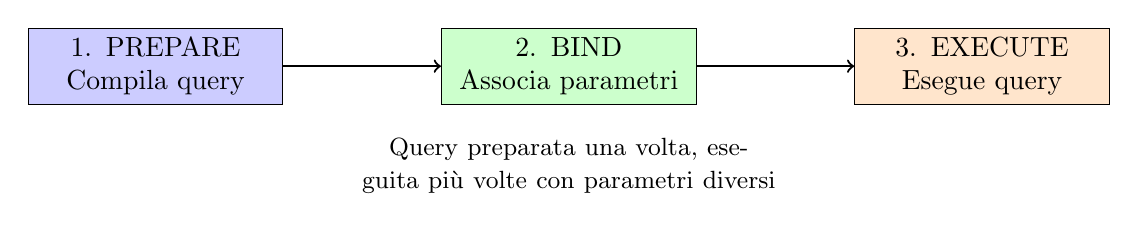
\begin{tikzpicture}[node distance=2cm]
				\node[rectangle, draw, fill=blue!20, text width=3cm, align=center] (prep) {1. PREPARE\\Compila query};
				\node[rectangle, draw, fill=green!20, text width=3cm, align=center, right=of prep] (bind) {2. BIND\\Associa parametri};
				\node[rectangle, draw, fill=orange!20, text width=3cm, align=center, right=of bind] (exec) {3. EXECUTE\\Esegue query};
				
				\draw[->, thick] (prep) -- (bind);
				\draw[->, thick] (bind) -- (exec);
				
				\node[below=0.3cm of bind, text width=8cm, align=center] {
					\small Query preparata una volta, eseguita più volte con parametri diversi
				};
			\end{tikzpicture}
		\end{center}
		
		\vspace{0.5cm}
		\textbf{Vantaggi}:
		\begin{itemize}
			\item \textcolor{red}{\textbf{Sicurezza}}: Previene SQL Injection
			\item \textcolor{blue}{\textbf{Performance}}: Query pre-compilata
			\item \textcolor{green}{\textbf{Chiarezza}}: Codice più leggibile
		\end{itemize}
	\end{frame}
	
	% Slide 15
	\begin{frame}[fragile]{prepare() ed execute()}
		\textbf{Sintassi base}:
		
		\begin{lstlisting}
			<?php
			// 1. PREPARE - con placeholder ?
			$sql = "SELECT * FROM studenti WHERE classe = ?";
			$stmt = $pdo->prepare($sql);
			
			// 2. EXECUTE - passa parametri
			$stmt->execute(['3A']);
			
			// 3. FETCH - recupera risultati
			$risultati = $stmt->fetchAll();
			
			foreach ($risultati as $studente) {
				echo $studente['nome'] . " " . $studente['cognome'];
			}
			?>
		\end{lstlisting}
	\end{frame}
	
	% Slide 16
	\begin{frame}[fragile]{Placeholder Posizionali (?)}
		\begin{lstlisting}
			<?php
			$sql = "SELECT * FROM studenti 
			WHERE classe = ? AND voto >= ?";
			
			$stmt = $pdo->prepare($sql);
			
			// L'ordine dei parametri DEVE corrispondere
			$stmt->execute(['3A', 7]);
			
			// Esempio con INSERT
			$sql = "INSERT INTO studenti (nome, cognome, classe) 
			VALUES (?, ?, ?)";
			$stmt = $pdo->prepare($sql);
			$stmt->execute(['Mario', 'Rossi', '3A']);
			?>
		\end{lstlisting}
		
		\alert{\textbf{Pro}}: Più compatti\\
		\alert{\textbf{Contro}}: Ordine critico, meno leggibile
	\end{frame}
	
	% Slide 17
	\begin{frame}[fragile]{Placeholder Nominativi (:nome)}
		\begin{lstlisting}
			<?php
			$sql = "SELECT * FROM studenti 
			WHERE classe = :classe AND voto >= :voto_min";
			
			$stmt = $pdo->prepare($sql);
			
			// Array associativo - ordine non importante!
			$stmt->execute([
			':classe' => '3A',
			':voto_min' => 7
			]);
			
			// Oppure senza i due punti nelle chiavi
			$stmt->execute([
			'classe' => '3A',
			'voto_min' => 7
			]);
			?>
		\end{lstlisting}
		
		\alert{\textbf{Raccomandato}}: Più leggibile e meno soggetto a errori
	\end{frame}
	
	% Slide 18
	\begin{frame}[fragile]{execute() con Array}
		\begin{lstlisting}
			<?php
			// INSERT multipli
			$sql = "INSERT INTO studenti (nome, cognome, classe) 
			VALUES (:nome, :cognome, :classe)";
			$stmt = $pdo->prepare($sql);
			
			$studenti = [
			['nome' => 'Mario', 'cognome' => 'Rossi', 'classe' => '3A'],
			['nome' => 'Laura', 'cognome' => 'Bianchi', 'classe' => '3A'],
			['nome' => 'Giuseppe', 'cognome' => 'Verdi', 'classe' => '3B']
			];
			
			foreach ($studenti as $studente) {
				$stmt->execute($studente);
			}
			
			echo "Inseriti " . count($studenti) . " studenti";
			?>
		\end{lstlisting}
	\end{frame}
	
	% SEZIONE 5: bindParam e bindValue
	\section{Binding dei Parametri}
	
	% Slide 19
	\begin{frame}[fragile]{bindValue() - Base}
		\textbf{Associa un valore a un parametro}:
		
		\begin{lstlisting}
			<?php
			$sql = "SELECT * FROM studenti WHERE classe = :classe";
			$stmt = $pdo->prepare($sql);
			
			// Binding singolo
			$stmt->bindValue(':classe', '3A');
			$stmt->execute();
			
			// Equivalente a:
			// $stmt->execute([':classe' => '3A']);
			?>
		\end{lstlisting}
		
		Utile quando:
		\begin{itemize}
			\item Si ha bisogno di controllo fine sui tipi
			\item Si costruisce la query dinamicamente
		\end{itemize}
	\end{frame}
	
	% Slide 20
	\begin{frame}[fragile]{bindParam() vs bindValue()}
		\begin{columns}
			\column{0.48\textwidth}
			\textbf{bindValue()} - per valore
			\begin{lstlisting}[basicstyle=\ttfamily\tiny]
				$classe = '3A';
				$stmt->bindValue(':c', $classe);
				$classe = '3B'; // Non influisce
				$stmt->execute();
				// Query con '3A'
			\end{lstlisting}
			
			\column{0.48\textwidth}
			\textbf{bindParam()} - per riferimento
			\begin{lstlisting}[basicstyle=\ttfamily\tiny]
				$classe = '3A';
				$stmt->bindParam(':c', $classe);
				$classe = '3B'; // Cambia!
				$stmt->execute();
				// Query con '3B'
			\end{lstlisting}
		\end{columns}
		
		\vspace{0.5cm}
		\begin{tcolorbox}[colback=blue!5,colframe=blue!40!black]
			\textbf{bindParam()} passa la variabile per riferimento - il valore viene letto al momento di \texttt{execute()}!
		\end{tcolorbox}
	\end{frame}
	
	% Slide 21
	\begin{frame}[fragile]{bindParam() - Esempio Pratico}
		\begin{lstlisting}
			<?php
			$sql = "INSERT INTO log (utente, azione, timestamp) 
			VALUES (:utente, :azione, :ts)";
			$stmt = $pdo->prepare($sql);
			
			// Binding per riferimento
			$stmt->bindParam(':utente', $utente);
			$stmt->bindParam(':azione', $azione);
			$stmt->bindParam(':ts', $timestamp);
			
			// Esecuzione multipla con valori diversi
			$utente = 'mario'; $azione = 'login'; 
			$timestamp = time();
			$stmt->execute();
			
			$utente = 'laura'; $azione = 'logout'; 
			$timestamp = time();
			$stmt->execute();
			?>
		\end{lstlisting}
	\end{frame}
	
	% Slide 22
	\begin{frame}[fragile]{Tipi di Dati (PDO::PARAM\_*)}
		\begin{lstlisting}
			<?php
			$sql = "SELECT * FROM studenti 
			WHERE voto >= :voto AND attivo = :attivo";
			$stmt = $pdo->prepare($sql);
			
			// Specificare il tipo esplicitamente
			$stmt->bindValue(':voto', 6, PDO::PARAM_INT);
			$stmt->bindValue(':attivo', true, PDO::PARAM_BOOL);
			
			$stmt->execute();
			?>
		\end{lstlisting}
		
		\textbf{Tipi disponibili}:
		\begin{itemize}
			\item \texttt{PDO::PARAM\_INT} - Intero
			\item \texttt{PDO::PARAM\_BOOL} - Booleano
			\item \texttt{PDO::PARAM\_STR} - Stringa (default)
			\item \texttt{PDO::PARAM\_NULL} - NULL
			\item \texttt{PDO::PARAM\_LOB} - Large Object
		\end{itemize}
	\end{frame}
	
	% SEZIONE 6: Metodi Fetch
	\section{Recupero Dati}
	
	% Slide 23
	\begin{frame}[fragile]{fetch() - Recupero Riga Singola}
		\begin{lstlisting}
			<?php
			$sql = "SELECT * FROM studenti WHERE id = :id";
			$stmt = $pdo->prepare($sql);
			$stmt->execute(['id' => 1]);
			
			// Recupera UNA riga
			$studente = $stmt->fetch();
			
			if ($studente) {
				echo $studente['nome'] . " " . $studente['cognome'];
			} else {
				echo "Studente non trovato";
			}
			?>
		\end{lstlisting}
		
		\textbf{Comportamento}:
		\begin{itemize}
			\item Prima chiamata: prima riga
			\item Seconda chiamata: seconda riga
			\item Nessuna riga: \texttt{false}
		\end{itemize}
	\end{frame}
	
	% Slide 24
	\begin{frame}[fragile]{fetch() in Loop}
		\begin{lstlisting}
			<?php
			$sql = "SELECT nome, cognome, voto FROM studenti 
			WHERE classe = '3A'";
			$stmt = $pdo->query($sql);
			
			// Ciclo su tutte le righe
			while ($riga = $stmt->fetch()) {
				echo $riga['nome'] . " " . $riga['cognome'];
				echo " - Voto: " . $riga['voto'] . "<br>";
			}
			?>
		\end{lstlisting}
		
		\vspace{0.3cm}
		\textbf{Vantaggio}: Consuma poca memoria anche con molti risultati\\
		\textbf{Quando usarlo}: Elaborazione riga per riga, grandi dataset
	\end{frame}
	
	% Slide 25
	\begin{frame}[fragile]{fetchAll() - Tutte le Righe}
		\begin{lstlisting}
			<?php
			$sql = "SELECT * FROM studenti WHERE classe = '3A'";
			$stmt = $pdo->query($sql);
			
			// Recupera TUTTE le righe in un array
			$studenti = $stmt->fetchAll();
			
			echo "Trovati " . count($studenti) . " studenti<br>";
			
			foreach ($studenti as $studente) {
				echo $studente['nome'] . "<br>";
			}
			?>
		\end{lstlisting}
		
		\textbf{Quando usarlo}:
		\begin{itemize}
			\item Risultati piccoli/medi
			\item Serve contare le righe prima di elaborarle
			\item Serve accesso random ai risultati
		\end{itemize}
	\end{frame}
	
	% Slide 26
	\begin{frame}[fragile]{Modalità di Fetch}
		\textbf{PDO::FETCH\_ASSOC} - Array associativo
		\begin{lstlisting}[basicstyle=\ttfamily\tiny]
			$row = $stmt->fetch(PDO::FETCH_ASSOC);
			// ['nome' => 'Mario', 'cognome' => 'Rossi']
		\end{lstlisting}
		
		\textbf{PDO::FETCH\_NUM} - Array numerico
		\begin{lstlisting}[basicstyle=\ttfamily\tiny]
			$row = $stmt->fetch(PDO::FETCH_NUM);
			// [0 => 'Mario', 1 => 'Rossi']
		\end{lstlisting}
		
		\textbf{PDO::FETCH\_BOTH} - Entrambi (default)
		\begin{lstlisting}[basicstyle=\ttfamily\tiny]
			$row = $stmt->fetch(PDO::FETCH_BOTH);
			// ['nome' => 'Mario', 0 => 'Mario', 'cognome' => 'Rossi', 1 => 'Rossi']
		\end{lstlisting}
		
		\alert{\textbf{Raccomandazione}}: Usare \texttt{FETCH\_ASSOC} per chiarezza
	\end{frame}
	
	% Slide 27
	\begin{frame}[fragile]{FETCH\_OBJ - Oggetto}
		\begin{lstlisting}
			<?php
			$sql = "SELECT * FROM studenti WHERE id = 1";
			$stmt = $pdo->query($sql);
			
			// Recupera come oggetto stdClass
			$studente = $stmt->fetch(PDO::FETCH_OBJ);
			
			echo $studente->nome;       // Proprietà, non chiavi!
			echo $studente->cognome;
			echo $studente->classe;
			?>
		\end{lstlisting}
		
		\vspace{0.3cm}
		Utile per:
		\begin{itemize}
			\item Accesso a proprietà con \texttt{->} invece di \texttt{[]}
			\item Integrazione con codice OOP
			\item IDE con autocompletamento
		\end{itemize}
	\end{frame}
	
	% Slide 28
	\begin{frame}[fragile]{FETCH\_CLASS - Oggetto Personalizzato}
		\begin{lstlisting}
			<?php
			class Studente {
				public $id;
				public $nome;
				public $cognome;
				
				public function nomeCompleto() {
					return $this->nome . " " . $this->cognome;
				}
			}
			
			$sql = "SELECT * FROM studenti WHERE classe = '3A'";
			$stmt = $pdo->query($sql);
			
			// Popola oggetti della classe Studente
			$studenti = $stmt->fetchAll(PDO::FETCH_CLASS, 'Studente');
			
			foreach ($studenti as $s) {
				echo $s->nomeCompleto();  // Usa metodo della classe!
			}
			?>
		\end{lstlisting}
	\end{frame}
	
	% Slide 29
	\begin{frame}[fragile]{fetchColumn() - Singola Colonna}
		\begin{lstlisting}
			<?php
			// Recupera solo una colonna
			$sql = "SELECT COUNT(*) FROM studenti";
			$stmt = $pdo->query($sql);
			$totale = $stmt->fetchColumn();
			echo "Totale studenti: $totale";
			
			// Recupera colonna specifica (0-based)
			$sql = "SELECT nome, cognome FROM studenti LIMIT 1";
			$stmt = $pdo->query($sql);
			$nome = $stmt->fetchColumn(0);    // Prima colonna
			$cognome = $stmt->fetchColumn(1); // Seconda colonna
			
			// Utile per liste
			$sql = "SELECT nome FROM studenti";
			$stmt = $pdo->query($sql);
			while ($nome = $stmt->fetchColumn()) {
				echo $nome . "<br>";
			}
			?>
		\end{lstlisting}
	\end{frame}
	
	% Slide 30
	\begin{frame}[fragile]{Impostare Fetch Mode Predefinito}
		\begin{lstlisting}
			<?php
			// Metodo 1: Alla connessione
			$options = [
			PDO::ATTR_DEFAULT_FETCH_MODE => PDO::FETCH_ASSOC
			];
			$pdo = new PDO($dsn, $user, $pass, $options);
			
			// Metodo 2: Dopo la connessione
			$pdo->setAttribute(
			PDO::ATTR_DEFAULT_FETCH_MODE, 
			PDO::FETCH_ASSOC
			);
			
			// Ora fetch() usa FETCH_ASSOC di default
			$stmt = $pdo->query("SELECT * FROM studenti");
			$studente = $stmt->fetch(); // Automaticamente ASSOC
			?>
		\end{lstlisting}
	\end{frame}
	
	% SEZIONE 7: SQL Injection
	\section{Prevenzione SQL Injection}
	
	% Slide 31
	\begin{frame}{Cos'è SQL Injection?}
		\begin{tcolorbox}[colback=red!10,colframe=red!80!black,title=\faExclamationTriangle~SQL Injection]
			Tecnica di attacco che sfrutta input non validati per iniettare codice SQL malevolo in una query.
		\end{tcolorbox}
		
		\vspace{0.3cm}
		\textbf{Conseguenze}:
		\begin{itemize}
			\item \textcolor{red}{Furto di dati sensibili}
			\item \textcolor{red}{Modifica/cancellazione dati}
			\item \textcolor{red}{Bypass autenticazione}
			\item \textcolor{red}{Esecuzione comandi sul server}
			\item \textcolor{red}{Compromissione totale del sistema}
		\end{itemize}
		
		\vspace{0.3cm}
		\alert{È uno dei 10 rischi più critici secondo OWASP!}
	\end{frame}
	
	% Slide 32
	\begin{frame}[fragile]{Esempio di Vulnerabilità}
		\begin{tcolorbox}[colback=red!20,colframe=red!80!black,title=\faTimes~CODICE VULNERABILE - MAI FARE COSÌ!]
			\begin{lstlisting}
				<?php
				// PERICOLOSO! Non usare concatenazione!
				$username = $_POST['username'];
				$password = $_POST['password'];
				
				$sql = "SELECT * FROM utenti 
				WHERE username = '$username' 
				AND password = '$password'";
				
				$result = $pdo->query($sql);
				?>
			\end{lstlisting}
		\end{tcolorbox}
		
		\textbf{Input malevolo}:
		\begin{verbatim}
			username: admin' OR '1'='1
			password: qualsiasi
		\end{verbatim}
		
	\end{frame}
	
	
		% Slide 32
	\begin{frame}[fragile]{Esempio di Vulnerabilità}
		
		\textbf{Input malevolo}:
		\begin{verbatim}
			username: admin' OR '1'='1
			password: qualsiasi
		\end{verbatim}
		
		\textbf{Query risultante}:
		\begin{verbatim}
			SELECT * FROM utenti WHERE username = 'admin' 
			OR '1'='1' AND password = 'qualsiasi'
		\end{verbatim}
	\end{frame}
	
	
	
	
	% Slide 33
	\begin{frame}[fragile]{Attacco SQL Injection - Diagramma}
		\begin{center}
			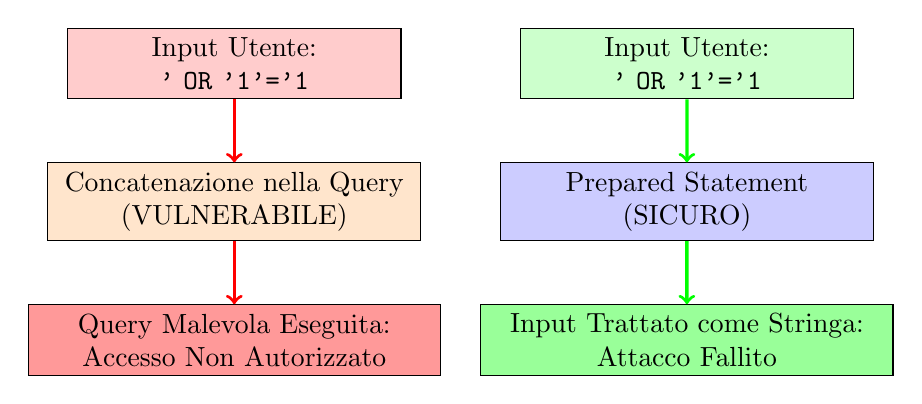
\begin{tikzpicture}[scale=0.85]
				\node[rectangle, draw, fill=red!20, text width=4cm, align=center] (input) {Input Utente:\\\texttt{' OR '1'='1}};
				\node[rectangle, draw, fill=orange!20, text width=4.5cm, align=center, below=0.8cm of input] (concat) {Concatenazione nella Query\\(VULNERABILE)};
				\node[rectangle, draw, fill=red!40, text width=5cm, align=center, below=0.8cm of concat] (malicious) {Query Malevola Eseguita:\\Accesso Non Autorizzato};
				
				\draw[->, very thick, red] (input) -- (concat);
				\draw[->, very thick, red] (concat) -- (malicious);
				
				\node[right=1.5cm of input, rectangle, draw, fill=green!20, text width=4cm, align=center] (safe) {Input Utente:\\\texttt{' OR '1'='1}};
				\node[rectangle, draw, fill=blue!20, text width=4.5cm, align=center, below=0.8cm of safe] (prepared) {Prepared Statement\\(SICURO)};
				\node[rectangle, draw, fill=green!40, text width=5cm, align=center, below=0.8cm of prepared] (escaped) {Input Trattato come Stringa:\\Attacco Fallito};
				
				\draw[->, very thick, green] (safe) -- (prepared);
				\draw[->, very thick, green] (prepared) -- (escaped);
			\end{tikzpicture}
		\end{center}
	\end{frame}
	
	% Slide 34
	\begin{frame}[fragile]{Soluzione: Prepared Statements}
		\begin{tcolorbox}[colback=green!20,colframe=green!80!black,title=\faCheck~CODICE SICURO]
			\begin{lstlisting}
				<?php
				// SICURO! Usa prepared statements!
				$username = $_POST['username'];
				$password = $_POST['password'];
				
				$sql = "SELECT * FROM utenti 
				WHERE username = :username 
				AND password = :password";
				
				$stmt = $pdo->prepare($sql);
				$stmt->execute([
				'username' => $username,
				'password' => $password
				]);
				
				$utente = $stmt->fetch();
				?>
			\end{lstlisting}
		\end{tcolorbox}
		
		I prepared statements \textbf{separano} logica SQL da dati!
	\end{frame}
	
	% Slide 35
	\begin{frame}{Come PDO Previene SQL Injection}
		\begin{enumerate}
			\item \textbf{Separazione}: Query e dati viaggiano separati
			\item \textbf{Escape automatico}: PDO fa escape di caratteri speciali
			\item \textbf{Type checking}: Verifica i tipi di dato
			\item \textbf{Parametrizzazione}: I parametri non sono mai interpretati come SQL
		\end{enumerate}
		
		\vspace{0.5cm}
		\begin{center}
			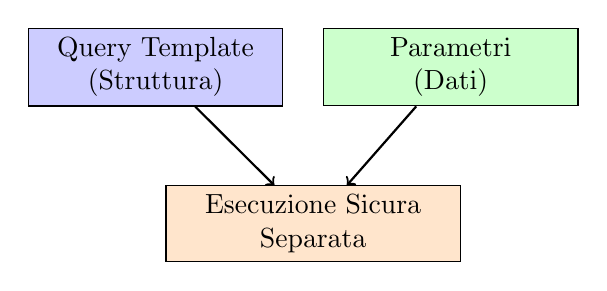
\begin{tikzpicture}
				\node[rectangle, draw, fill=blue!20, text width=3cm, align=center] (query) {Query Template\\(Struttura)};
				\node[rectangle, draw, fill=green!20, text width=3cm, align=center, right=0.5cm of query] (params) {Parametri\\(Dati)};
				\node[rectangle, draw, fill=orange!20, text width=3.5cm, align=center, below=1cm of query, xshift=2cm] (safe) {Esecuzione Sicura\\Separata};
				
				\draw[->, thick] (query) -- (safe);
				\draw[->, thick] (params) -- (safe);
			\end{tikzpicture}
		\end{center}
	\end{frame}
	
	% Slide 36
	\begin{frame}[fragile]{Best Practices di Sicurezza}
		\begin{tcolorbox}[colback=green!10,colframe=green!60!black,title=\faShieldAlt~Regole d'Oro]
			\begin{enumerate}
				\item \textbf{SEMPRE} usare prepared statements per input utente
				\item \textbf{MAI} concatenare SQL con variabili
				\item \textbf{MAI} usare \texttt{query()} con dati non fidati
				\item Validare input anche prima di PDO
				\item Usare \texttt{ERRMODE\_EXCEPTION}
				\item Non mostrare errori SQL all'utente finale
				\item Applicare principio del minimo privilegio (utente DB limitato)
				\item Hash delle password (mai in chiaro!)
			\end{enumerate}
		\end{tcolorbox}
	\end{frame}
	
	% Slide 37
	\begin{frame}[fragile]{Validazione Input (Difesa Aggiuntiva)}
		\begin{lstlisting}
			<?php
			// Validazione PRIMA di usare PDO
			$id = $_GET['id'];
			
			// Verifica che sia un numero
			if (!is_numeric($id) || $id < 1) {
				die("ID non valido");
			}
			
			// Cast esplicito
			$id = (int)$id;
			
			// Ora usalo nel prepared statement
			$sql = "SELECT * FROM studenti WHERE id = :id";
			$stmt = $pdo->prepare($sql);
			$stmt->execute(['id' => $id]);
			?>
		\end{lstlisting}
		
		\alert{Validazione + Prepared Statements = Difesa a Strati}
	\end{frame}
	
	% Slide 38
	\begin{frame}[fragile]{LIKE con Prepared Statements}
		\textbf{Problema}: Come usare LIKE in modo sicuro?
		
		\begin{lstlisting}
			<?php
			$cerca = $_GET['cerca'];
			
			// SBAGLIATO: pattern nella query
			// $sql = "SELECT * FROM studenti WHERE nome LIKE '%$cerca%'";
			
			// GIUSTO: pattern nel parametro
			$sql = "SELECT * FROM studenti WHERE nome LIKE :pattern";
			$stmt = $pdo->prepare($sql);
			
			$pattern = "%{$cerca}%";  // Costruisci pattern in PHP
			$stmt->execute(['pattern' => $pattern]);
			
			$risultati = $stmt->fetchAll();
			?>
		\end{lstlisting}
		
		\alert{Il carattere \% va nei DATI, non nella query!}
	\end{frame}
	
	% SEZIONE 8: Transazioni
	\section{Transazioni}
	
	% Slide 39
	\begin{frame}{Cos'è una Transazione?}
		\begin{tcolorbox}[colback=blue!10,colframe=blue!60!black,title=Transazione]
			Gruppo di operazioni SQL trattate come \textbf{un'unica unità atomica}: o si completano tutte con successo, o nessuna ha effetto.
		\end{tcolorbox}
		
		\vspace{0.3cm}
		\textbf{Proprietà ACID}:
		\begin{description}
			\item[Atomicity] Tutto o niente
			\item[Consistency] Dati consistenti
			\item[Isolation] Transazioni indipendenti
			\item[Durability] Modifiche permanenti
		\end{description}
		
		\vspace{0.3cm}
		\textbf{Esempio}: Trasferimento bancario
		\begin{itemize}
			\item Sottrai da conto A
			\item Aggiungi a conto B
			\item Se una fallisce, annulla tutto!
		\end{itemize}
	\end{frame}
	
	% Slide 40
	\begin{frame}[fragile]{Sintassi Base delle Transazioni}
		\begin{lstlisting}
			<?php
			try {
				// 1. INIZIO transazione
				$pdo->beginTransaction();
				
				// 2. OPERAZIONI multiple
				$stmt1 = $pdo->prepare("UPDATE conti SET saldo = saldo - 100 WHERE id = 1");
				$stmt1->execute();
				
				$stmt2 = $pdo->prepare("UPDATE conti SET saldo = saldo + 100 WHERE id = 2");
				$stmt2->execute();
				
				// 3. COMMIT - conferma tutto
				$pdo->commit();
				echo "Trasferimento completato";
				
			} catch (Exception $e) {
				// 4. ROLLBACK - annulla tutto
				$pdo->rollBack();
				echo "Errore: " . $e->getMessage();
			}
			?>
		\end{lstlisting}
	\end{frame}
	
%	% Slide 41
%	\begin{frame}{Flusso di una Transazione}
%		\begin{center}
%			\begin{tikzpicture}[node distance=1.5cm]
%				\node[rectangle, draw, fill=blue!20, rounded corners] (begin) {beginTransaction()};
%				\node[rectangle, draw, fill=yellow!20, rounded corners, below=of begin] (op1) {Operazione 1};
%				\node[rectangle, draw, fill=yellow!20, rounded corners, below=of op1] (op2) {Operazione 2};
%				\node[rectangle, draw, fill=yellow!20, rounded corners, below=of op2] (op3) {Operazione N};
%				\node[diamond, draw, fill=orange!20, aspect=2, below=of op3] (check) {Errore?};
%				\node[rectangle, draw, fill=green!40, rounded corners, below left=1cm and 0.5cm of check] (commit) {commit()\\Conferma};
%				\node[rectangle, draw, fill=red!40, rounded corners, below right=1cm and 0.5cm of check] (rollback) {rollBack()\\Annulla};
%				
%				\draw[->, thick] (begin) -- (op1);
%				\draw[->, thick] (op1) -- (op2);
%				\draw[->, thick] (op2) -- (op3);
%				\draw[->, thick] (op3) -- (check);
%				\draw[->, thick] (check) -- node[left] {NO} (commit);
%				\draw[->, thick] (check) -- node[right] {SI} (rollback);
%			\end{tikzpicture}
%		\end{center}
%	\end{frame}
	
	% Slide 42
	\begin{frame}[fragile]{commit() - Conferma Modifiche}
		\begin{lstlisting}
			<?php
			$pdo->beginTransaction();
			
			// Inserimento multiplo
			$sql = "INSERT INTO ordini (cliente, totale) 
			VALUES (:cliente, :totale)";
			$stmt = $pdo->prepare($sql);
			
			$stmt->execute(['cliente' => 'Mario', 'totale' => 150]);
			$ordineId = $pdo->lastInsertId();
			
			$sql = "INSERT INTO dettagli_ordine (ordine_id, prodotto) 
			VALUES (:ordine, :prodotto)";
			$stmt = $pdo->prepare($sql);
			$stmt->execute(['ordine' => $ordineId, 'prodotto' => 'Laptop']);
			
			// Tutto ok, conferma!
			$pdo->commit();
			echo "Ordine salvato con successo!";
			?>
		\end{lstlisting}
		
		\alert{commit() rende le modifiche \textbf{permanenti}}
	\end{frame}
	
	% Slide 43
	\begin{frame}[fragile]{rollBack() - Annulla Modifiche}
		\begin{lstlisting}
			<?php
			try {
				$pdo->beginTransaction();
				
				// Prima operazione
				$pdo->exec("UPDATE prodotti SET quantita = quantita - 1 
				WHERE id = 5");
				
				// Simula errore
				if (/* condizione errore */) {
					throw new Exception("Stock insufficiente");
				}
				
				// Seconda operazione
				$pdo->exec("INSERT INTO vendite (prodotto_id) VALUES (5)");
				
				$pdo->commit();
				
			} catch (Exception $e) {
				// Annulla TUTTE le modifiche
				$pdo->rollBack();
				echo "Vendita annullata: " . $e->getMessage();
			}
			?>
		\end{lstlisting}
	\end{frame}
	
	% Slide 44
	\begin{frame}[fragile]{Verifica Stato Transazione}
		\begin{lstlisting}
			<?php
			// Controlla se c'e' una transazione attiva
			if ($pdo->inTransaction()) {
				echo "Transazione in corso";
			} else {
				echo "Nessuna transazione";
			}
			
			// Esempio pratico
			try {
				$pdo->beginTransaction();
				
				// ... operazioni ...
				
				if ($pdo->inTransaction()) {
					$pdo->commit();
				}
				
			} catch (Exception $e) {
				if ($pdo->inTransaction()) {
					$pdo->rollBack();
				}
			}
			?>
		\end{lstlisting}
	\end{frame}
	
	% Slide 45
	\begin{frame}[fragile]{Transazioni Annidate (Savepoint)}
		\begin{lstlisting}
			<?php
			try {
				$pdo->beginTransaction();
				
				// Prima operazione
				$pdo->exec("INSERT INTO log VALUES ('operazione 1')");
				
				// Savepoint
				$pdo->exec("SAVEPOINT sp1");
				
				// Seconda operazione
				$pdo->exec("INSERT INTO log VALUES ('operazione 2')");
				
				// Errore! Torna al savepoint
				$pdo->exec("ROLLBACK TO SAVEPOINT sp1");
				
				// Commit (salva solo operazione 1)
				$pdo->commit();
				
			} catch (Exception $e) {
				$pdo->rollBack();
			}
			?>
		\end{lstlisting}
		
		\small\alert{Nota}: Supporto savepoint dipende dal DBMS
	\end{frame}
	
	% Slide 46
	\begin{frame}{Quando Usare le Transazioni}
		\textbf{Usare transazioni per}:
		\begin{itemize}
			\item[\faCheck] Operazioni finanziarie (pagamenti, trasferimenti)
			\item[\faCheck] Inserimenti correlati su più tabelle
			\item[\faCheck] Aggiornamenti che devono essere atomici
			\item[\faCheck] Operazioni con vincoli di integrità complessi
			\item[\faCheck] Batch di operazioni che devono completare insieme
		\end{itemize}
		
		\vspace{0.3cm}
		\textbf{Non necessarie per}:
		\begin{itemize}
			\item[\faTimes] Singole SELECT
			\item[\faTimes] Operazioni indipendenti
			\item[\faTimes] Log non critici
		\end{itemize}
		
		\vspace{0.3cm}
		\alert{Regola: Se un'operazione dipende dal successo di un'altra, usa transazioni!}
	\end{frame}
	
	% SEZIONE 9: Gestione Errori
	\section{Gestione Errori Avanzata}
	
	% Slide 47
	\begin{frame}[fragile]{Try-Catch Completo}
		\begin{lstlisting}
			<?php
			try {
				$pdo = new PDO($dsn, $user, $pass, [
				PDO::ATTR_ERRMODE => PDO::ERRMODE_EXCEPTION
				]);
				
				$stmt = $pdo->prepare("SELECT * FROM studenti WHERE id = :id");
				$stmt->execute(['id' => $id]);
				$studente = $stmt->fetch();
				
				if (!$studente) {
					throw new Exception("Studente non trovato");
				}
				
			} catch (PDOException $e) {
				// Errore PDO specifico
				error_log("Errore DB: " . $e->getMessage());
				die("Errore nel database");
				
			} catch (Exception $e) {
				// Altri errori
				error_log("Errore: " . $e->getMessage());
				die("Errore nell'applicazione");
			}
			?>
		\end{lstlisting}
	\end{frame}
	
	% Slide 48
	\begin{frame}[fragile]{Informazioni sugli Errori}
		\begin{lstlisting}
			<?php
			try {
				$stmt = $pdo->prepare("SELECT * FROM tabella_inesistente");
				$stmt->execute();
				
			} catch (PDOException $e) {
				echo "Messaggio: " . $e->getMessage() . "<br>";
				echo "Codice: " . $e->getCode() . "<br>";
				echo "File: " . $e->getFile() . "<br>";
				echo "Linea: " . $e->getLine() . "<br>";
				
				// SQLSTATE e codice errore MySQL
				echo "SQLSTATE: " . $e->errorInfo[0] . "<br>";
				echo "Codice errore: " . $e->errorInfo[1] . "<br>";
				echo "Messaggio DB: " . $e->errorInfo[2] . "<br>";
			}
			?>
		\end{lstlisting}
		
		\alert{In produzione: loggare gli errori, non mostrarli all'utente!}
	\end{frame}
	
	% Slide 49
	\begin{frame}[fragile]{Logging degli Errori}
		\begin{lstlisting}
			<?php
			// Funzione di logging personalizzata
			function logError($e) {
				$log = date('Y-m-d H:i:s') . " - ";
				$log .= "SQLSTATE: " . $e->errorInfo[0] . " - ";
				$log .= $e->getMessage() . "\n";
				
				file_put_contents(
				'logs/db_errors.log', 
				$log, 
				FILE_APPEND
				);
			}
			
			try {
				// ... operazioni DB ...
			} catch (PDOException $e) {
				logError($e);
				
				// Messaggio generico all'utente
				die("Si è verificato un errore. Riprova più tardi.");
			}
			?>
		\end{lstlisting}
	\end{frame}
	
	% SEZIONE 10: Best Practices
	\section{Best Practices}
	
	% Slide 50
	\begin{frame}{Riepilogo Best Practices}
		\begin{enumerate}
			\item \textbf{Connessione}
			\begin{itemize}
				\item Usare \texttt{ERRMODE\_EXCEPTION}
				\item Impostare \texttt{charset=utf8mb4}
				\item Disabilitare emulazione prepared statements
			\end{itemize}
			
			\item \textbf{Sicurezza}
			\begin{itemize}
				\item SEMPRE prepared statements per input utente
				\item MAI concatenazione SQL
				\item Validare input
				\item Non mostrare errori SQL all'utente
			\end{itemize}
			
			\item \textbf{Performance}
			\begin{itemize}
				\item Usare \texttt{fetch()} per dataset grandi
				\item Riutilizzare prepared statements in loop
				\item Chiudere connessioni quando non servono
			\end{itemize}
		\end{enumerate}
	\end{frame}
	
	% Slide 51
	\begin{frame}{Checklist Finale}
		\begin{tcolorbox}[colback=green!10,colframe=green!60!black,title=\faCheckSquare~Checklist PDO]
			\begin{itemize}
				\item[$\square$] Modalità errore su EXCEPTION
				\item[$\square$] Charset UTF-8 (utf8mb4)
				\item[$\square$] Prepared statements per query parametrizzate
				\item[$\square$] Placeholder nominativi (:nome) per chiarezza
				\item[$\square$] Gestione errori con try-catch
				\item[$\square$] Transazioni per operazioni atomiche
				\item[$\square$] Logging errori (non visualizzati all'utente)
				\item[$\square$] Validazione input
				\item[$\square$] Hash password (password\_hash/verify)
				\item[$\square$] Principio minimo privilegio per utente DB
			\end{itemize}
		\end{tcolorbox}
	\end{frame}
	
	% Slide 52
	\begin{frame}{Risorse Utili}
		\textbf{Documentazione Ufficiale}:
		\begin{itemize}
			\item \url{https://www.php.net/manual/en/book.pdo.php}
			\item \url{https://www.php.net/manual/en/pdo.prepared-statements.php}
		\end{itemize}
		
		\vspace{0.3cm}
		\textbf{Sicurezza}:
		\begin{itemize}
			\item OWASP - SQL Injection Prevention
			\item PHP The Right Way - Database
		\end{itemize}
		
		\vspace{0.3cm}
		\textbf{Best Practices}:
		\begin{itemize}
			\item PHP-FIG Standards (PSR-12)
			\item MySQL Performance Best Practices
		\end{itemize}
	\end{frame}
	
	% Slide 53
	\begin{frame}[fragile]{Esempio Completo - Applicazione CRUD}
		\begin{lstlisting}[basicstyle=\ttfamily\tiny]
			<?php
			class StudenteDAO {
				private $pdo;
				
				public function __construct($pdo) {
					$this->pdo = $pdo;
				}
				
				public function inserisci($nome, $cognome, $classe) {
					$sql = "INSERT INTO studenti (nome, cognome, classe) 
					VALUES (:nome, :cognome, :classe)";
					$stmt = $this->pdo->prepare($sql);
					$stmt->execute([
					'nome' => $nome,
					'cognome' => $cognome,
					'classe' => $classe
					]);
					return $this->pdo->lastInsertId();
				}
				
				public function leggiTutti() {
					$sql = "SELECT * FROM studenti ORDER BY cognome, nome";
					$stmt = $this->pdo->query($sql);
					return $stmt->fetchAll(PDO::FETCH_ASSOC);
				}
			\end{lstlisting}
		\end{frame}
		
		% Slide 54
		\begin{frame}[fragile]{Esempio Completo - Continuazione}
			\begin{lstlisting}[basicstyle=\ttfamily\tiny]
				public function leggiPerId($id) {
					$sql = "SELECT * FROM studenti WHERE id = :id";
					$stmt = $this->pdo->prepare($sql);
					$stmt->execute(['id' => $id]);
					return $stmt->fetch(PDO::FETCH_ASSOC);
				}
				
				public function aggiorna($id, $nome, $cognome, $classe) {
					$sql = "UPDATE studenti 
					SET nome = :nome, cognome = :cognome, classe = :classe 
					WHERE id = :id";
					$stmt = $this->pdo->prepare($sql);
					return $stmt->execute([
					'id' => $id,
					'nome' => $nome,
					'cognome' => $cognome,
					'classe' => $classe
					]);
				}
				
				public function elimina($id) {
					$sql = "DELETE FROM studenti WHERE id = :id";
					$stmt = $this->pdo->prepare($sql);
					return $stmt->execute(['id' => $id]);
				}
			}
			?>
		\end{lstlisting}
	\end{frame}
	
	% Slide 55 - Conclusione
	\begin{frame}{Conclusioni}
		\begin{center}
			\Large\textbf{PDO: La Scelta Giusta per PHP Moderno}
		\end{center}
		
		\vspace{0.5cm}
		\textbf{Abbiamo visto}:
		\begin{itemize}
			\item Connessione sicura e configurata
			\item Prepared statements per sicurezza
			\item Metodi fetch per recupero dati
			\item Transazioni per integrità
			\item Prevenzione SQL Injection
			\item Best practices di sviluppo
		\end{itemize}
		
		\vspace{0.5cm}
		\begin{center}
			\textcolor{darkblue}{\textbf{Grazie per l'attenzione!}}
			
			\vspace{0.3cm}
			\small
			Domande?\\
			\texttt{massimo.pippi@ferrmi-ceci.edu.it}
		\end{center}
	\end{frame}
	
\end{document}